\documentclass[titlepage]{article}
\usepackage{listings}
\lstMakeShortInline{|}
\usepackage{courier}
%\usepackage{hyperref}
\usepackage[colorlinks,linkcolor=blue,citecolor=blue,urlcolor=blue,breaklinks=true]{hyperref}
\lstset{basicstyle=\ttfamily\small , breaklines}
%\usepackage[margin=2cm]{geometry}
\usepackage[left=3cm,top=3cm,bottom=3cm, right=3cm,includehead,includefoot,landscape]{geometry}
\usepackage{color}
\usepackage{fancyhdr,lastpage}
\pagestyle{fancy}
\rhead{Metrum Research Group, LLC \\ }
\lhead{
\includegraphics[scale=2]{logo.png}}
\cfoot{Page \thepage\ of \pageref{LastPage}}
\fancyhfoffset{.25in}
\renewcommand{\headrulewidth}{0.25pt}
\renewcommand{\footrulewidth}{0pt} 
\setlength{\headheight}{23pt}
\renewcommand{\labelitemiii}{$\circ$}
\usepackage{longtable}
\usepackage{amsmath}
\usepackage[T1]{fontenc}
\usepackage[scaled]{helvet}
\renewcommand*\familydefault{\sfdefault}
\usepackage{courier}
\usepackage{graphicx}
\usepackage{tocbibind}
\usepackage[parfill]{parskip}    % Activate to begin paragraphs with an empty line rather than an indent
\usepackage{upgreek}
\usepackage{textpos}
\usepackage{relsize}
\usepackage{upquote}
% Use \begin{landscape} and end{landscape} to rotate text %%%
\usepackage{pdflscape}
\usepackage{textcomp}
\usepackage{float}
\floatplacement{figure}{H}
\floatplacement{table}{H}
\usepackage[printonlyused,nohyperlinks]{acronym}
\def\bflabel#1{{\large#1\ \ \ \ }\hfill}
\usepackage{fixltx2e}
\setlength{\belowcaptionskip}{10pt}





\usepackage{Sweave}

 
\begin{document}
\vspace*{2cm}
\begin{center}
{\Large Covariate Plots}\\
~\\
\today\\
~\\
Tim Bergsma\\
\end{center}
\newpage

\section{Purpose}
This script picks up after model.Rnw to process bootstrap results and make covariate plots.
\subsection{Summarize bootstrap models.}
\begin{Schunk}
\begin{Sinput}
> #wait for bootstraps to finish
> getwd()
\end{Sinput}
\begin{Soutput}
[1] "/data/metrumrg/inst/example/project/script"
\end{Soutput}
\begin{Sinput}
> require(metrumrg)
> boot <- read.csv('../nonmem/1005bootlog.csv',as.is=TRUE)
> head(boot)
\end{Sinput}
\begin{Soutput}
  X tool run parameter   moment            value
1 1  nm7   1       ofv  minimum 2459.17577376723
2 2  nm7   1    THETA1 estimate          9.90624
3 3  nm7   1    THETA1     prse             <NA>
4 4  nm7   1    THETA1       se             <NA>
5 5  nm7   1    THETA2 estimate          21.8851
6 6  nm7   1    THETA2     prse             <NA>
\end{Soutput}
\begin{Sinput}
> unique(boot$parameter)
\end{Sinput}
\begin{Soutput}
 [1] "ofv"      "THETA1"   "THETA2"   "THETA3"   "THETA4"   "THETA5"  
 [7] "THETA6"   "THETA7"   "OMEGA1.1" "OMEGA2.1" "OMEGA2.2" "OMEGA3.1"
[13] "OMEGA3.2" "OMEGA3.3" "SIGMA1.1" "SIGMA2.1" "SIGMA2.2" "cov"     
[19] "prob"     "min"      "data"    
\end{Soutput}
\begin{Sinput}
> text2decimal(unique(boot$parameter))
\end{Sinput}
\begin{Soutput}
 [1]  NA 1.0 2.0 3.0 4.0 5.0 6.0 7.0 1.1 2.1 2.2 3.1 3.2 3.3 1.1 2.1 2.2  NA  NA
[20]  NA  NA
\end{Soutput}
\begin{Sinput}
> boot$X <- NULL
\end{Sinput}
\end{Schunk}
It looks like we have 14 estimated parameters.  We will map them to the
original control stream.
\begin{Schunk}
\begin{Sinput}
> boot <- boot[!is.na(text2decimal(boot$parameter)),]
> head(boot)
\end{Sinput}
\begin{Soutput}
  tool run parameter   moment   value
2  nm7   1    THETA1 estimate 9.90624
3  nm7   1    THETA1     prse    <NA>
4  nm7   1    THETA1       se    <NA>
5  nm7   1    THETA2 estimate 21.8851
6  nm7   1    THETA2     prse    <NA>
7  nm7   1    THETA2       se    <NA>
\end{Soutput}
\begin{Sinput}
> unique(boot$moment)
\end{Sinput}
\begin{Soutput}
[1] "estimate" "prse"     "se"      
\end{Soutput}
\begin{Sinput}
> unique(boot$value[boot$moment=='prse'])
\end{Sinput}
\begin{Soutput}
[1] NA
\end{Soutput}
\end{Schunk}
prse, and therefore moment, is noninformative for these bootstraps.
\begin{Schunk}
\begin{Sinput}
> boot <- boot[boot$moment=='estimate',]
> boot$moment <- NULL
> unique(boot$tool)
\end{Sinput}
\begin{Soutput}
[1] "nm7"
\end{Soutput}
\begin{Sinput}
> boot$tool <- NULL
> head(boot)
\end{Sinput}
\begin{Soutput}
   run parameter     value
2    1    THETA1   9.90624
5    1    THETA2   21.8851
8    1    THETA3 0.0708172
11   1    THETA4   3.36908
14   1    THETA5   94.6441
17   1    THETA6  0.972459
\end{Soutput}
\begin{Sinput}
> unique(boot$value[boot$parameter %in% c('OMEGA2.1','OMEGA3.1','OMEGA3.2')])
\end{Sinput}
\begin{Soutput}
  [1] "0.118664"     "0.00243903"   "-0.0290796"   "0.126793"     "0.00496538"  
  [6] "-0.0348756"   "0.0793827"    "0.0126369"    "-0.0254598"   "0.0930785"   
 [11] "-0.00800534"  "-0.0604644"   "0.0776862"    "-0.033206"    "-0.0431809"  
 [16] "0.103253"     "-0.00112888"  "-0.0399964"   "0.124331"     "-0.00239167" 
 [21] "-0.029284"    "0.0929814"    "0.00605676"   "-0.0318726"   "0.127233"    
 [26] "0.0107017"    "-0.0244607"   "0.112805"     "0.0269056"    "-0.00833839" 
 [31] "0.089781"     "0.00380984"   "-0.0419745"   "0.145258"     "-0.0511888"  
 [36] "-0.034809"    "0.123498"     "0.0100472"    "-0.0206121"   "0.087605"    
 [41] "-0.0100154"   "-0.0246587"   "0.0852641"    "-0.00160618"  "-0.0344951"  
 [46] "0.130004"     "0.0285763"    "-0.0412472"   "0.0885414"    "-0.00653594" 
 [51] "-0.0477025"   "0.128072"     "-0.043122"    "-0.0414366"   "0.0643089"   
 [56] "-0.0278958"   "-0.0369344"   "0.190185"     "-0.0205086"   "-0.0254147"  
 [61] "0.118594"     "-0.00752878"  "-0.0254214"   "0.0984033"    "-0.0268537"  
 [66] "-0.0508149"   "0.128197"     "0.0232717"    "-0.0236485"   "0.167161"    
 [71] "-0.0217378"   "-0.0381076"   "0.165581"     "0.0026395"    "-0.0201113"  
 [76] "0.0947898"    "-0.0169356"   "-0.0396992"   "0.0463237"    "-0.00590113" 
 [81] "-0.0567564"   "0.194381"     "-0.016843"    "-0.0245055"   "0.104522"    
 [86] "0.00451787"   "-0.0224597"   "0.106576"     "-0.0108525"   "-0.0250716"  
 [91] "0.108904"     "-0.011186"    "-0.0269199"   "0.099795"     "-0.0395158"  
 [96] "-0.0396872"   "0.0850945"    "-0.0237444"   "-0.0408458"   "0.118145"    
[101] "-0.0351339"   "-0.0617783"   "0.11275"      "-0.0256919"   "-0.0452783"  
[106] "0.238867"     "0.0421175"    "-0.0113238"   "0.14246"      "-0.0102745"  
[111] "-0.024625"    "0.177373"     "0.0528303"    "0.00958209"   "0.106911"    
[116] "0.0084715"    "-0.0370734"   "0.0610869"    "-0.0328259"   "-0.047843"   
[121] "0.144278"     "0.00445557"   "-0.0430449"   "0.132424"     "-0.00549815" 
[126] "-0.0287111"   "0.0982603"    "-0.000319022" "-0.0017437"   "0.171037"    
[131] "0.0245733"    "-0.000645002" "0.0966426"    "-0.0427972"   "-0.0422852"  
[136] "0.104497"     "-0.00685035"  "-0.0241402"   "0.048328"     "-0.0161035"  
[141] "-0.0432615"   "0.10326"      "0.00876954"   "-0.0425963"   "0.0835945"   
[146] "-0.000345751" "-0.0447939"   "0.112744"     "0.00295217"   "-0.038452"   
[151] "0.179544"     "0.0253114"    "-0.0173357"   "0.0567234"    "0.00397885"  
[156] "-0.0299795"   "0.180876"     "-0.00185961"  "-0.0249431"   "0.117222"    
[161] "0.0146515"    "-0.0264576"   "0.0867059"    "-0.0341638"   "-0.0468783"  
[166] "0.161077"     "0.016314"     "0.00365817"   "0.110393"     "-0.0199048"  
[171] "-0.0610041"   "0.0933731"    "0.00429235"   "-0.0585371"   "0.131606"    
[176] "-0.0273357"   "-0.0414518"   "0.0740837"    "-0.0393725"   "-0.0532824"  
[181] "0.114816"     "0.000498657"  "-0.0327203"   "0.166113"     "0.0260557"   
[186] "-0.0135421"   "0.202143"     "0.0177433"    "-0.0210063"   "0.0910233"   
[191] "0.0151667"    "-0.0408356"   "0.0869677"    "0.0132545"    "-0.0369345"  
[196] "0.121655"     "-0.0174125"   "-0.0312738"   "0.117305"     "-0.00249383" 
[201] "-0.0312059"   "0.0697088"    "-0.0238347"   "-0.0435523"   "0.157214"    
[206] "0.0276361"    "-0.0167383"   "0.103765"     "-0.0320889"   "-0.0491544"  
[211] "0.127115"     "0.00963291"   "-0.0315352"   "0.109701"     "-0.00298642" 
[216] "-0.0269827"   "0.16388"      "-0.0222152"   "-0.0279416"   "0.149759"    
[221] "-0.0606384"   "-0.0582305"   "0.156684"     "-0.00684425"  "-0.012883"   
[226] "0.132933"     "0.0117935"    "-0.0325854"   "0.0667252"    "-0.0396604"  
[231] "-0.0444942"   "0.16451"      "0.00956835"   "-0.0156386"   "0.09734"     
[236] "-0.00795721"  "-0.0377005"   "0.114314"     "-0.00645326"  "-0.0362318"  
[241] "0.130343"     "-0.0293751"   "-0.0610221"   "0.146619"     "-0.000407232"
[246] "-0.0189186"   "0.137891"     "0.000284756"  "-0.0289554"   "0.0894687"   
[251] "-0.045893"    "-0.0433736"   "0.146665"     "0.0142544"    "-0.0046038"  
[256] "0.128874"     "0.00757832"   "-0.0270146"   "0.173957"     "0.0191542"   
[261] "-0.0231056"   "0.105145"     "-0.0287821"   "-0.0461986"   "0.174007"    
[266] "-0.0250103"   "-0.0154687"   "0.157456"     "-0.024208"    "-0.0433639"  
[271] "0.11283"      "-0.0196416"   "-0.0358259"   "0.110391"     "-0.0343518"  
[276] "-0.0621958"   "0.119436"     "0.00084654"   "-0.0184177"   "0.0932988"   
[281] "-0.0145868"   "-0.0412257"   "0.11698"      "-0.0102802"   "-0.0421815"  
[286] "0.12102"      "-0.0340955"   "-0.0461667"   "0.204833"     "0.0048392"   
[291] "-0.0163318"   "0.102249"     "-0.0446726"   "-0.041768"    "0.100408"    
[296] "-0.018728"    "-0.0527315"   "0.105437"     "-0.0330352"   "-0.0412061"  
[301] "0.133189"     "-0.0168328"   "-0.0265733"   "0.0945628"    "-0.023821"   
[306] "-0.046713"    "0.115873"     "-0.0174054"   "-0.0383742"   "0.151988"    
[311] "-0.00223515"  "-0.0378195"   "0.111794"     "-0.0362"      "-0.0342003"  
[316] "0.115686"     "-0.0487321"   "-0.060517"    "0.0491857"    "-0.0400171"  
[321] "-0.0577105"   "0.0924036"    "-0.00301072"  "-0.0217227"   "0.120695"    
[326] "-0.0180271"   "-0.0419004"   "0.0841407"    "-0.0272724"   "-0.0373296"  
[331] "0.139445"     "-0.0562157"   "-0.0628584"   "0.133837"     "-0.00586549" 
[336] "-0.0465415"   "0.117258"     "0.00585337"   "-0.0212932"   "0.141695"    
[341] "-0.0128164"   "-0.0454878"   "0.0762841"    "-0.0419415"   "-0.0446022"  
[346] "0.115743"     "-0.0270675"   "-0.0334311"   "0.138236"     "0.0159711"   
[351] "-0.0182158"   "0.153652"     "-0.0133617"   "-0.0312735"   "0.129189"    
[356] "-0.00427277"  "-0.0375778"   "0.0784215"    "-0.0189919"   "-0.0278138"  
[361] "0.0859258"    "-0.0112918"   "-0.0467703"   "0.152543"     "-0.0117078"  
[366] "-0.0259285"   "0.146407"     "-0.00833509"  "-0.034062"    "0.117961"    
[371] "-0.0228667"   "-0.0302872"   "0.0998222"    "-0.0056598"   "-0.0270215"  
[376] "0.148139"     "-0.0358078"   "-0.0466091"   "0.154802"     "-0.00387405" 
[381] "-0.0344275"   "0.0821857"    "0.0179231"    "-0.0208862"   "0.159922"    
[386] "-0.00843248"  "-0.0361851"   "0.154326"     "-0.0204394"   "-0.0313897"  
[391] "0.0876006"    "0.0186169"    "-0.0384454"   "0.145707"     "-0.0513646"  
[396] "-0.0353279"   "0.0960684"    "-0.0153064"   "-0.0325897"   "0.11394"     
[401] "-0.034478"    "-0.0391465"   "0.120386"     "-0.0235295"   "-0.0403019"  
[406] "0.146429"     "-0.00908831"  "-0.0229428"   "0.097815"     "-0.0228671"  
[411] "-0.0477668"   "0.0527412"    "-0.0401556"   "-0.0404198"   "0.191292"    
[416] "0.0233172"    "0.00230111"   "0.0966339"    "-0.0101169"   "-0.0304393"  
[421] "0.10204"      "-0.0675111"   "-0.0323571"   "0.0669481"    "-0.00414325" 
[426] "-0.0350418"   "0.117326"     "0.0193662"    "-0.0293494"   "0.043366"    
[431] "-0.037891"    "-0.0554599"   "0.116669"     "-0.0318554"   "-0.0605897"  
[436] "0.0694246"    "-0.0246743"   "-0.0545532"   "0.0898996"    "-0.0190038"  
[441] "-0.0526655"   "0.115324"     "-0.0447849"   "-0.043447"    "0.121016"    
[446] "-0.00117652"  "-0.0408539"   "0.0741252"    "-0.018944"    "-0.0254045"  
[451] "0.104378"     "-0.00161247"  "-0.02001"     "0.157005"     "-0.00523794" 
[456] "-0.0247991"   "0.353326"     "0.0462137"    "0.00466421"   "0.118066"    
[461] "-0.0221416"   "-0.0276645"   "0.114712"     "-0.00405465"  "-0.0277673"  
[466] "0.12592"      "-0.0129521"   "-0.0347467"   "0.0982355"    "0.011252"    
[471] "-0.0208779"   "0.069048"     "-0.0578171"   "-0.0478397"   "0.116005"    
[476] "-0.0531913"   "-0.0461022"   "0.189958"     "0.023425"     "-0.00411602" 
[481] "0.0874002"    "-0.0666577"   "-0.0453464"   "0.2505"       "0.0077027"   
[486] "-0.020866"    "0.167599"     "0.0451788"    "-0.000658309" "0.102168"    
[491] "-0.0143335"   "-0.0314068"   "0.0899941"    "-0.0436014"   "-0.0577496"  
[496] "0.0724949"    "-0.0250441"   "-0.0245517"   "0.105756"     "-0.0395233"  
[501] "-0.031799"    "0.11358"      "0.0199425"    "-0.0149443"   "0.0744656"   
[506] "-0.067681"    "-0.0450863"   "0.0890981"    "-0.0412376"   "-0.0493254"  
[511] "0.114138"     "-0.0385923"   "-0.0430469"   "0.0888011"    "-0.0233544"  
[516] "-0.0528061"   "0.0437555"    "-0.0220735"   "-0.0363112"   "0.108748"    
[521] "-0.00845016"  "-0.0437129"   "0.0888528"    "-0.027201"    "-0.0455558"  
[526] "0.109073"     "0.0282737"    "-0.0144904"   "0.129467"     "-0.00760702" 
[531] "-0.0198483"   "0.124009"     "0.0141844"    "-0.0382784"   "0.0587984"   
[536] "-0.0244563"   "-0.0366547"   "0.151268"     "-0.00472393"  "-0.0293829"  
[541] "0.174939"     "-0.00865166"  "-0.0339589"   "0.156336"     "-0.0134474"  
[546] "-0.0319209"   "0.146133"     "-0.0145848"   "-0.020574"    "0.146571"    
[551] "-0.014698"    "-0.0412586"   "0.164571"     "-0.0107431"   "-0.0206866"  
[556] "0.080354"     "-0.021482"    "-0.0432427"   "0.112315"     "-0.0225172"  
[561] "-0.0452995"   "0.182548"     "-0.0240036"   "-0.0307118"   "0.148057"    
[566] "-0.00531287"  "-0.0421696"   "0.10471"      "0.00909549"   "-0.0103994"  
[571] "0.141531"     "-0.0117441"   "-0.0268305"   "0.0559151"    "-0.0145141"  
[576] "-0.0399355"   "0.28593"      "0.0647187"    "0.0090289"    "0.226196"    
[581] "0.0465617"    "-0.0167024"   "0.0863951"    "-0.0242882"   "-0.0445673"  
[586] "0.106766"     "0.00711912"   "-0.0384497"   "0.128791"     "0.00935973"  
[591] "-0.0255152"   "0.151827"     "0.0441323"    "0.00135172"   "0.112872"    
[596] "-0.00344834"  "-0.022351"    "0.0481444"    "-0.0179546"   "-0.055449"   
[601] "0.0818587"    "-0.0253594"   "-0.0342839"   "0.0963877"    "-0.00883704" 
[606] "-0.0304148"   "0.139391"     "-0.0187507"   "-0.0402836"   "0.155405"    
[611] "-0.010436"    "-0.0216516"   "0.0635618"    "-0.00394322"  "-0.0362427"  
[616] "0.134236"     "0.0036363"    "-0.00675133"  "0.0945227"    "-0.0698679"  
[621] "-0.0602625"   "0.0923165"    "-0.0150991"   "-0.03504"     "0.081674"    
[626] "-0.00441006"  "-0.0490822"   "0.128433"     "-0.0261758"   "-0.0399649"  
[631] "0.109765"     "-0.0263731"   "-0.0386598"   "0.0884195"    "0.0352562"   
[636] "-0.0224681"   "0.125047"     "-0.0162158"   "-0.0186845"   "0.0836961"   
[641] "0.00447476"   "-0.0381655"   "0.113755"     "0.0275129"    "-0.00949459" 
[646] "0.0651323"    "-0.0287285"   "-0.0593339"   "0.12926"      "-0.0386841"  
[651] "-0.0235969"   "0.1418"       "0.00185295"   "-0.0213206"   "0.113659"    
[656] "-0.0188672"   "-0.0347941"   "0.0657834"    "-0.0261605"   "-0.0511768"  
[661] "0.119641"     "-0.0109612"   "-0.0345783"   "0.107459"     "-0.0279097"  
[666] "-0.0412287"   "0.128837"     "-0.00841091"  "-0.0275248"   "0.0641978"   
[671] "-0.0448828"   "-0.0548623"   "0.105479"     "-0.00756979"  "-0.0405812"  
[676] "0.171147"     "0.00200281"   "-0.0121898"   "0.0862844"    "-0.0229536"  
[681] "-0.0273754"   "0.183258"     "0.00836453"   "-0.0156531"   "0.0791151"   
[686] "-0.0363597"   "-0.04549"     "0.233874"     "0.00370539"   "-0.0186613"  
[691] "0.142951"     "-0.0015608"   "-0.0336835"   "0.0595705"    "-0.0238448"  
[696] "-0.0408746"   "0.0778225"    "-0.0396712"   "-0.0301179"   "0.0918823"   
[701] "-0.0157737"   "-0.0291893"   "0.112115"     "0.0144137"    "-0.0306044"  
[706] "0.138055"     "-0.0309795"   "-0.043204"    "0.138132"     "0.00912759"  
[711] "-0.033212"    "0.138767"     "-0.0134388"   "-0.0507434"   "0.124444"    
[716] "-0.047932"    "-0.0479316"   "0.171497"     "-0.0121706"   "-0.0242095"  
[721] "0.0539906"    "-0.0110564"   "-0.0497779"   "0.0957407"    "-0.0272087"  
[726] "-0.0377266"   "0.105232"     "-0.0423657"   "-0.0309091"   "0.0727366"   
[731] "-0.00618372"  "-0.042519"    "0.140173"     "-0.0588466"   "-0.0585394"  
[736] "0.1177"       "-0.0279011"   "-0.0488746"   "0.141545"     "0.0282797"   
[741] "-0.00360611"  "0.150651"     "0.0033684"    "-0.0222497"   "0.141123"    
[746] "-0.0345764"   "-0.0358508"   "0.126262"     "0.00663914"   "-0.0317031"  
[751] "0.127498"     "-0.0124166"   "-0.0283863"   "0.131374"     "-0.0134399"  
[756] "-0.036174"    "0.148283"     "-0.0190479"   "-0.017962"    "0.12113"     
[761] "-0.0326466"   "-0.0519758"   "0.115299"     "-0.0400513"   "-0.0586101"  
[766] "0.153765"     "-0.00778942"  "-0.0310329"   "0.0721597"    "-0.0137686"  
[771] "-0.0349912"   "0.106628"     "0.00160757"   "-0.0459419"   "0.13816"     
[776] "-0.0181902"   "-0.0264274"   "0.0938884"    "-0.0191998"   "-0.0385028"  
[781] "0.146527"     "-0.00176887"  "-0.0262183"   "0.0941695"    "0.00247702"  
[786] "-0.0389381"   "0.153674"     "0.0248971"    "0.00316929"   "0.135013"    
[791] "-0.0159761"   "-0.0366188"   "0.150773"     "-0.0121322"   "-0.0210345"  
[796] "0.100948"     "-0.0100324"   "-0.0380679"   "0.0781693"    "-0.0131155"  
[801] "-0.0260249"   "0.183728"     "0.0471509"    "-0.00331759"  "0.122793"    
[806] "0.0128808"    "-0.022205"    "0.0961981"    "0.00881522"   "-0.0339731"  
[811] "0.0988059"    "0.0129752"    "-0.0250672"   "0.106903"     "-0.0307499"  
[816] "-0.0488798"   "0.199369"     "-0.0026988"   "-0.034997"    "0.103321"    
[821] "0.0245504"    "-0.00192493"  "0.106192"     "0.00493618"   "-0.0361149"  
[826] "0.0844764"    "0.00496454"   "-0.0254247"   "0.058592"     "-0.00590223" 
[831] "-0.0442436"   "0.0701997"    "-0.00732918"  "-0.0466255"   "0.0715442"   
[836] "-0.0347355"   "-0.0415529"   "0.0926783"    "-0.0344959"   "-0.0327224"  
[841] "0.121309"     "-0.0321942"   "-0.0385079"   "0.099353"     "0.000595448" 
[846] "-0.0240711"   "0.149399"     "-0.0155101"   "-0.041984"    "0.158858"    
[851] "0.0105719"    "-0.00492554"  "0.067364"     "-0.0108857"   "-0.0470531"  
[856] "0.127813"     "0.00669009"   "-0.0184069"   "0.14897"      "0.0134118"   
[861] "-0.0248284"   "0.135642"     "0.0179566"    "-0.00793688"  "0.060602"    
[866] "0.00193913"   "-0.0211142"   "0.0592927"    "-0.0327238"   "-0.0356362"  
[871] "0.136618"     "-0.0223643"   "-0.0262968"   "0.106394"     "-0.0196676"  
[876] "-0.0533358"   "0.0742905"    "-0.00833212"  "-0.0373445"   "0.0998197"   
[881] "-0.00384365"  "-0.025143"    "0.170587"     "-0.0143729"   "-0.0394337"  
[886] "0.0868"       "-0.0287056"   "-0.0297065"   "0.100429"     "0.00791036"  
[891] "-0.0297891"   "0.059776"     "-0.0391323"   "-0.0377099"   "0.112937"    
[896] "0.00219594"   "-0.0172751"   "0.174089"     "0.0131627"    "-0.0141584"  
\end{Soutput}
\begin{Sinput}
> unique(boot$parameter[boot$value=='0'])
\end{Sinput}
\begin{Soutput}
[1] "SIGMA2.1"
\end{Soutput}
\end{Schunk}
Off-diagonals (and only off-diagonals) are noninformative.
\begin{Schunk}
\begin{Sinput}
> boot <- boot[!boot$value=='0',]
> any(is.na(as.numeric(boot$value)))
\end{Sinput}
\begin{Soutput}
[1] FALSE
\end{Soutput}
\begin{Sinput}
> boot$value <- as.numeric(boot$value)
> head(boot)
\end{Sinput}
\begin{Soutput}
   run parameter      value
2    1    THETA1  9.9062400
5    1    THETA2 21.8851000
8    1    THETA3  0.0708172
11   1    THETA4  3.3690800
14   1    THETA5 94.6441000
17   1    THETA6  0.9724590
\end{Soutput}
\end{Schunk}
\subsection{Restrict data to 95 percentiles.}
We did 300 runs.  Min and max are strongly dependent on number of runs, since 
with an unbounded distribution, (almost) any value is possible with enough sampling.
We clip to the 95 percentiles, to give distributions that are somewhat more
scale independent.
\begin{Schunk}
\begin{Sinput}
> boot <- inner(
+ 	boot, 
+ 	preserve='run',
+ 	id.var='parameter',
+ 	measure.var='value'
+ )
> head(boot)
\end{Sinput}
\begin{Soutput}
  run parameter      value
1   1    THETA1  9.9062400
2   1    THETA2 21.8851000
3   1    THETA3  0.0708172
4   1    THETA4  3.3690800
5   1    THETA5 94.6441000
6   1    THETA6  0.9724590
\end{Soutput}
\begin{Sinput}
> any(is.na(boot$value))
\end{Sinput}
\begin{Soutput}
[1] TRUE
\end{Soutput}
\begin{Sinput}
> boot <- boot[!is.na(boot$value),]
\end{Sinput}
\end{Schunk}
\subsection{Recover parameter metadata from a specially-marked control stream.}
We want meaningful names for our parameters.  Harvest these from a reviewed control
stream.
\begin{Schunk}
\begin{Sinput}
> wiki <- wikitab(1005,'../nonmem')
> wiki
\end{Sinput}
\begin{Soutput}
   parameter                                   description
1     THETA1                       apparent oral clearance
2     THETA2                central volume of distribution
3     THETA3                      absorption rate constant
4     THETA4                  intercompartmental clearance
5     THETA5             peripheral volume of distribution
6     THETA6                      male effect on clearance
7     THETA7                    weight effect on clearance
8   OMEGA1.1      interindividual variability of clearance
9   OMEGA2.1   interindividual clearance-volume covariance
10  OMEGA2.2 interindividual variability of central volume
11  OMEGA3.1       interindividual clearance-Ka covariance
12  OMEGA3.2          interindividual volume-Ka covariance
13  OMEGA3.3             interindividual variability of Ka
14  SIGMA1.1                            proportional error
15  SIGMA2.2                                additive error
                                                                model tool  run
1  CL/F (L/h) ~ theta_1 *  theta_6 ^MALE * (WT/70)^theta_7  * e^eta_1  nm7 1005
2                          V_c /F (L) ~ theta_2 * (WT/70)^1 * e^eta_2  nm7 1005
3                                     K_a (h^-1 ) ~ theta_3 * e^eta_3  nm7 1005
4                                                 Q/F (L/h) ~ theta_4  nm7 1005
5                                                V_p /F (L) ~ theta_5  nm7 1005
6                                                 MALE_CL/F ~ theta_6  nm7 1005
7                                                   WT_CL/F ~ theta_7  nm7 1005
8                                                IIV_CL/F ~ Omega_1.1  nm7 1005
9                                                cov_CL,V ~ Omega_2.1  nm7 1005
10                                             IIV_V_c /F ~ Omega_2.2  nm7 1005
11                                             cov_CL,Ka  ~ Omega_3.1  nm7 1005
12                                              cov_V,Ka  ~ Omega_3.2  nm7 1005
13                                               IIV_K_a  ~ Omega_3.3  nm7 1005
14                                               err_prop ~ Sigma_1.1  nm7 1005
15                                                err_add ~ Sigma_2.2  nm7 1005
     estimate prse         se
1      9.5079 9.72   0.923845
2     22.7899 9.56    2.17804
3   0.0714253 7.34 0.00524566
4      3.4739 15.4   0.535313
5     113.258 20.9    23.6434
6     1.02445   11   0.112909
7     1.19194 28.3   0.337219
8    0.213815 22.8  0.0488441
9    0.120753 26.4  0.0319031
10  0.0945159 33.2  0.0313359
11 -0.0115975  173  0.0200682
12 -0.0371806 36.1  0.0134303
13  0.0465513 34.8   0.016184
14  0.0491672 10.9  0.0053805
15   0.201823 33.5  0.0675911
\end{Soutput}
\begin{Sinput}
> wiki$name <- wiki2label(wiki$model)
> wiki$estimate <- as.numeric(wiki$estimate)
> unique(wiki$parameter)
\end{Sinput}
\begin{Soutput}
 [1] "THETA1"   "THETA2"   "THETA3"   "THETA4"   "THETA5"   "THETA6"  
 [7] "THETA7"   "OMEGA1.1" "OMEGA2.1" "OMEGA2.2" "OMEGA3.1" "OMEGA3.2"
[13] "OMEGA3.3" "SIGMA1.1" "SIGMA2.2"
\end{Soutput}
\begin{Sinput}
> unique(boot$parameter)
\end{Sinput}
\begin{Soutput}
 [1] "THETA1"   "THETA2"   "THETA3"   "THETA4"   "THETA5"   "THETA6"  
 [7] "THETA7"   "OMEGA1.1" "OMEGA2.1" "OMEGA2.2" "OMEGA3.1" "OMEGA3.2"
[13] "OMEGA3.3" "SIGMA1.1" "SIGMA2.2"
\end{Soutput}
\begin{Sinput}
> boot <- stableMerge(boot, wiki[,c('parameter','name')])
> head(boot)
\end{Sinput}
\begin{Soutput}
  run parameter      value      name
1   1    THETA1  9.9062400      CL/F
2   1    THETA2 21.8851000     V_c/F
3   1    THETA3  0.0708172       K_a
4   1    THETA4  3.3690800       Q/F
5   1    THETA5 94.6441000     V_p/F
6   1    THETA6  0.9724590 MALE_CL/F
\end{Soutput}
\end{Schunk}
\subsection{Create covariate plot.}
Now we make a covariate plot for clearance.  We will normalize clearance 
by its median (we also could have used the model estimate).  We need to take 
cuts of weight, since we can only really show categorically-constrained distributions.
Male effect is already categorical.  I.e, the reference individual has median
clearance, is female, and has median weight.
\subsubsection{Recover original covariates for guidance.}
\begin{Schunk}
\begin{Sinput}
> covariates <- read.csv('../data/derived/phase1.csv',na.strings='.')
> head(covariates)
\end{Sinput}
\begin{Soutput}
     C ID TIME SEQ EVID  AMT    DV SUBJ HOUR HEIGHT WEIGHT SEX  AGE DOSE FED
1    C  1 0.00   0    0   NA 0.000    1 0.00    174   74.2   0 29.1 1000   1
2 <NA>  1 0.00   1    1 1000    NA    1 0.00    174   74.2   0 29.1 1000   1
3 <NA>  1 0.25   0    0   NA 0.363    1 0.25    174   74.2   0 29.1 1000   1
4 <NA>  1 0.50   0    0   NA 0.914    1 0.50    174   74.2   0 29.1 1000   1
5 <NA>  1 1.00   0    0   NA 1.120    1 1.00    174   74.2   0 29.1 1000   1
6 <NA>  1 2.00   0    0   NA 2.280    1 2.00    174   74.2   0 29.1 1000   1
  SMK DS CRCN TAFD  TAD LDOS MDV predose zerodv
1   0  0 83.5 0.00   NA   NA   0       1      0
2   0  0 83.5 0.00 0.00 1000   1       0      0
3   0  0 83.5 0.25 0.25 1000   0       0      0
4   0  0 83.5 0.50 0.50 1000   0       0      0
5   0  0 83.5 1.00 1.00 1000   0       0      0
6   0  0 83.5 2.00 2.00 1000   0       0      0
\end{Soutput}
\begin{Sinput}
> with(covariates,constant(WEIGHT,within=ID))
\end{Sinput}
\begin{Soutput}
[1] TRUE
\end{Soutput}
\begin{Sinput}
> covariates <- unique(covariates[,c('ID','WEIGHT')])
> head(covariates)
\end{Sinput}
\begin{Soutput}
   ID WEIGHT
1   1   74.2
16  2   80.3
31  3   94.2
46  4   85.2
61  5   82.8
76  6   63.9
\end{Soutput}
\begin{Sinput}
> covariates$WT <- as.numeric(covariates$WEIGHT)
> wt <- median(covariates$WT)
> wt
\end{Sinput}
\begin{Soutput}
[1] 81
\end{Soutput}
\begin{Sinput}
> range(covariates$WT)
\end{Sinput}
\begin{Soutput}
[1]  61 117
\end{Soutput}
\end{Schunk}
\subsubsection{Reproduce the control stream submodel for selective cuts of a continuous covariate.}
In the model we normalized by 70 kg, so that cut will have null effect.
Let's try 65, 75, and 85 kg. We have to make a separate column for each
cut, which is a bit of work. Basically, we make two more copies of our
weight effect columns, and raise our normalized cuts to those powers, 
effectively reproducing the submodel from the control stream.
\begin{Schunk}
\begin{Sinput}
> head(boot) 
\end{Sinput}
\begin{Soutput}
  run parameter      value      name
1   1    THETA1  9.9062400      CL/F
2   1    THETA2 21.8851000     V_c/F
3   1    THETA3  0.0708172       K_a
4   1    THETA4  3.3690800       Q/F
5   1    THETA5 94.6441000     V_p/F
6   1    THETA6  0.9724590 MALE_CL/F
\end{Soutput}
\begin{Sinput}
> unique(boot$name)
\end{Sinput}
\begin{Soutput}
 [1] "CL/F"      "V_c/F"     "K_a"       "Q/F"       "V_p/F"     "MALE_CL/F"
 [7] "WT_CL/F"   "IIV_CL/F"  "cov_CL,V"  "IIV_V_c/F" "cov_CL,Ka" "cov_V,Ka" 
[13] "IIV_K_a"   "err_prop"  "err_add"  
\end{Soutput}
\begin{Sinput}
> clearance <- boot[boot$name %in% c('CL/F','WT_CL/F','MALE_CL/F'),]
> head(clearance)
\end{Sinput}
\begin{Soutput}
   run parameter    value      name
1    1    THETA1 9.906240      CL/F
6    1    THETA6 0.972459 MALE_CL/F
7    1    THETA7 1.469340   WT_CL/F
16   2    THETA1 9.030570      CL/F
21   2    THETA6 1.038960 MALE_CL/F
22   2    THETA7 0.999512   WT_CL/F
\end{Soutput}
\begin{Sinput}
> frozen <- data.frame(cast(clearance,run~name),check.names=FALSE)
> head(frozen)
\end{Sinput}
\begin{Soutput}
  run     CL/F MALE_CL/F  WT_CL/F
1   1  9.90624  0.972459 1.469340
2   2  9.03057  1.038960 0.999512
3   3  9.33144  0.846678 1.909720
4   4  9.25626  0.940994 1.697690
5   5 10.27090  1.252490 1.159250
6   6  9.42006  0.967176 1.484520
\end{Soutput}
\begin{Sinput}
> frozen$`WT_CL/F:65` <- (65/70)**frozen$`WT_CL/F`
> frozen$`WT_CL/F:75` <- (75/70)**frozen$`WT_CL/F`
> frozen$`WT_CL/F:85` <- (85/70)**frozen$`WT_CL/F`
\end{Sinput}
\end{Schunk}
\subsubsection{Normalize key parameter}
\begin{Schunk}
\begin{Sinput}
> #cl <- median(boot$value[boot$name=='CL/F'])
> cl <- with(wiki, estimate[name=='CL/F'])
> cl
\end{Sinput}
\begin{Soutput}
[1] 9.5079
\end{Soutput}
\begin{Sinput}
> head(frozen)
\end{Sinput}
\begin{Soutput}
  run     CL/F MALE_CL/F  WT_CL/F WT_CL/F:65 WT_CL/F:75 WT_CL/F:85
1   1  9.90624  0.972459 1.469340  0.8968292   1.106690   1.330136
2   2  9.03057  1.038960 0.999512  0.9286050   1.071392   1.214171
3   3  9.33144  0.846678 1.909720  0.8680331   1.140831   1.448870
4   4  9.25626  0.940994 1.697690  0.8817803   1.124264   1.390435
5   5 10.27090  1.252490 1.159250  0.9176771   1.083265   1.252417
6   6  9.42006  0.967176 1.484520  0.8958209   1.107850   1.334062
\end{Soutput}
\begin{Sinput}
> frozen[['CL/F']] <- frozen[['CL/F']]/cl
> head(frozen)
\end{Sinput}
\begin{Soutput}
  run      CL/F MALE_CL/F  WT_CL/F WT_CL/F:65 WT_CL/F:75 WT_CL/F:85
1   1 1.0418957  0.972459 1.469340  0.8968292   1.106690   1.330136
2   2 0.9497965  1.038960 0.999512  0.9286050   1.071392   1.214171
3   3 0.9814407  0.846678 1.909720  0.8680331   1.140831   1.448870
4   4 0.9735336  0.940994 1.697690  0.8817803   1.124264   1.390435
5   5 1.0802491  1.252490 1.159250  0.9176771   1.083265   1.252417
6   6 0.9907614  0.967176 1.484520  0.8958209   1.107850   1.334062
\end{Soutput}
\begin{Sinput}
> frozen$`WT_CL/F` <- NULL
> molten <- melt(frozen,id.var='run',na.rm=TRUE)
> head(molten)
\end{Sinput}
\begin{Soutput}
  run variable     value
1   1     CL/F 1.0418957
2   2     CL/F 0.9497965
3   3     CL/F 0.9814407
4   4     CL/F 0.9735336
5   5     CL/F 1.0802491
6   6     CL/F 0.9907614
\end{Soutput}
\end{Schunk}
\subsubsection{Plot.}
Now we plot.  We reverse the variable factor to give us top-down layout
of strips.
\begin{Schunk}
\begin{Sinput}
> levels(molten$variable)
\end{Sinput}
\begin{Soutput}
[1] "CL/F"       "MALE_CL/F"  "WT_CL/F:65" "WT_CL/F:75" "WT_CL/F:85"
\end{Soutput}
\begin{Sinput}
> molten$variable <- factor(molten$variable,levels=rev(levels(molten$variable)))
> print(
+   stripplot(
+     variable~value,
+     data=molten,
+     panel=panel.covplot,
+     xlab=parse(text=with(wiki,wiki2plotmath(noUnits(model[name=='CL/F'])))),
+     main=with(wiki,description[name=='CL/F']),
+     sub=('(normalized)\n\n\n')
+   )
+ )
\end{Sinput}
\end{Schunk}
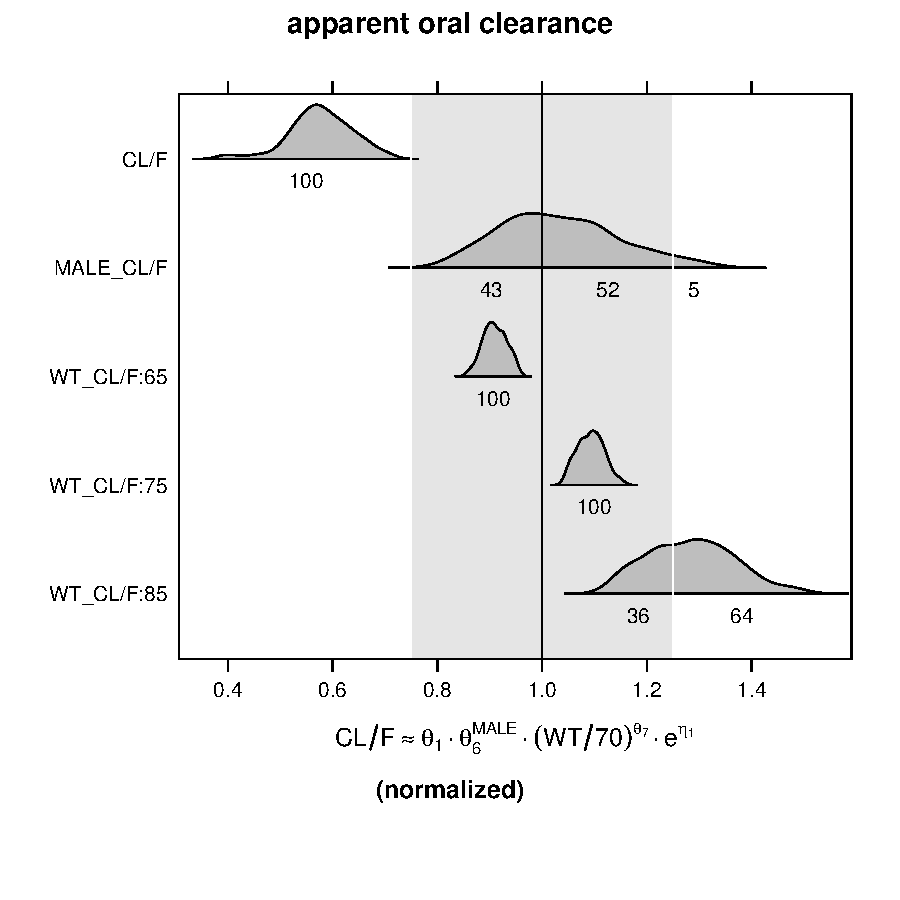
\includegraphics{covplot-covplot}
\subsubsection{Summarize}
We see that clearance is estimated with good precision.  Ignoring outliers, there 
is not much effect on clearance of being male, relative to female.  Increasing 
weight is associated with increasing clearance.  There is some probability
that an 85 kg person will have at least 25 percent greater clearance than a 70 kg
person.
\end{document}
